
	We want to compare the performance of the Steklov Scheme with simulations of the Stochastic
Lorenz System proposal in \cite{Keller1996}.
H. Keller. Attractors and bifurcations of the stochastic Lorenz system.
\begin{align}
	du &= (-Au - B(u) + f)dt +C(u)dW(t) \notag\\
	A & = 
	\begin{bmatrix}
		\sigma	&-\sigma	&0\\
		\sigma	&1			&0\\
		0		&0			&\beta
	\end{bmatrix}, 
	\qquad
	B(u) = 
	\begin{bmatrix}
		0\\
		xz\\
		-xy
	\end{bmatrix},
	\qquad
	f=
	\begin{bmatrix}
		0\\
		0\\
		-\beta(r+\sigma)
	\end{bmatrix} \label{eqn:LorenzSDE}\\
	C(u) &: \mathbb{R}^3 \to \mathbb{M}_{3 \times m}(\mathbb{R}), \qquad
	\|C(u)\|^2 = \Tr\left(C(u)C(u)^T\right)\leq K^2(1+ \|u\|^2).
	\notag
\end{align}
The simulations was performed with $C(u)=\sqrt{q}u$.
The following SSLS scheme gives good results.
\begin{align}
	a_1(y) &= \sigma y, \qquad a_2(x,z) = -x (\sigma +z) \qquad 
	a_3(x,y) = x y -\beta(\sigma +r) \notag\\
	X_{k+1} &= \exp(-\sigma h) X_{k}
		+\frac{a_1(Y_k)}{\sigma}
		(1-\exp(-\sigma h)), \notag\\
	Y_{k+1} &= a_2(X_{k+1},Z_{k}) (1-\exp(-h))
		+Y_k \exp(-h), \label{eqn:LorenzSSLS}\\
	Z_{k+1} &= \frac{a_3(X_{k+1}, Y_{k+1})}{\beta} (1- \exp(-\beta h))
		+Z_{k} \exp(-\beta h), \notag\\
	u_{k+1} &= (X_{k+1},Y_{k+1},Z_{k+1})^T + \sqrt{q} \Delta W_k (X_{k},Y_{k},Z_{k})^T.
	\notag
\end{align}

	In \Cref{fig:LorenzPaths} we present bought, deterministic and stochastic paths of Lorenz
SDE \Cref{eqn:LorenzSDE} produced by the \SM scheme \eqref{eqn:LorenzSSLS}. Also, in order to compare
the performance of the underlying scheme, in \Cref{fig:LorenzNumericalDis} we show the associated 
distribution of the last \num{1000} steps generated with the EM and \SM methods.
%
\begin{figure}[h!]
	\subfloat[Deterministic $q=\num{0}$.]{
		\centering
		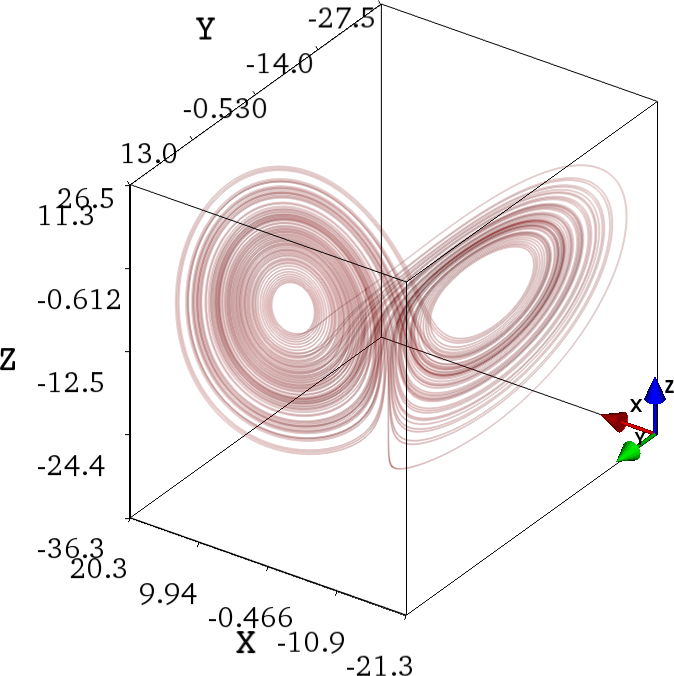
\includegraphics[width=0.45\linewidth]{./papers/paperB/figures/SDELorenz1.png}
		}
		\subfloat[Noise intensity $q = \num{0.3}$]{
			\centering
			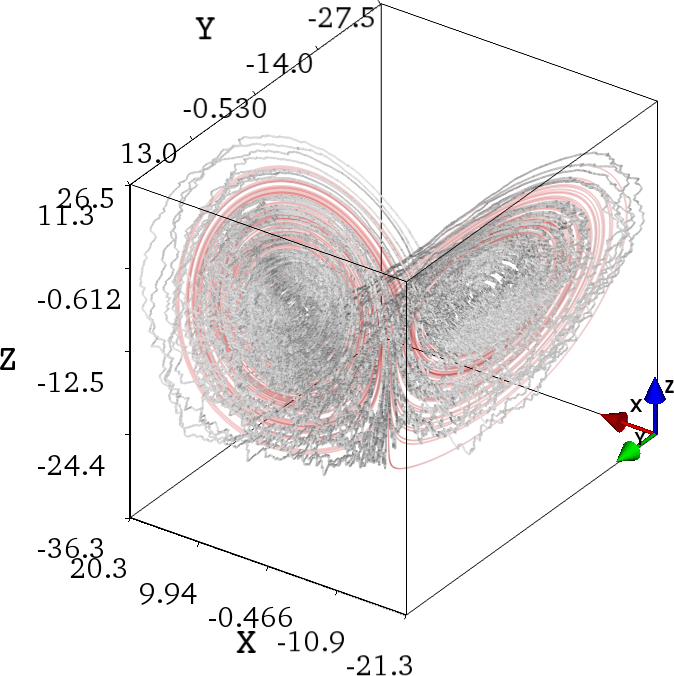
\includegraphics[width=0.45\linewidth]{./papers/paperB/figures/SDELorenz2.png}
		}
	\caption{Simulated paths of the Lorentz SDE \eqref{eqn:LorenzSDE} using the SSLS scheme
		\eqref{eqn:LorenzSSLS}. At the left the color red denotes the deterministic path with 
		$T = 100.0$,
		$h = \num{1e-06}$,
		$\sigma = \num{10.0}$,
		$\beta = \num{2.67}$,
		$\rho = \num{28.0}$,
		$U_0 = [\num{2.0}, \num{2.0}, \num{-9.0}]$.
		On the right, the gray color denotes the resulting path with same parameter and multiplicative 
		intensity $q = \num{0.3}$ noise.
	}\label{fig:LorenzPaths}
\end{figure}
\newgeometry{left=1.75cm, top=2cm, bottom=2cm}
\begin{figure}[htb]
	\centering
	\subfloat[EM $h=\num{1e-4}$.]{
		\includegraphics[width=0.4\textwidth]{./papers/paperB/figures/Histogram/EMDistributionh1.png}
		\label{subfig:EMDistLorenzSDE}
	}
	\subfloat[SSLS $h = \num{1e-4}$.]{
		\includegraphics[width=0.4\textwidth]{./papers/paperB/figures/Histogram/SSDistributionh1.png}
		\label{subfig:SSLSDistLorenzSDE}
	}\\
	\subfloat[EM $h=\num{1e-3}$.]{
		\includegraphics[width=0.4\textwidth]{./papers/paperB/figures/Histogram/EMDistributionh2.png}
		\label{subfig:EMDist2LorenzSDE}
	}
	\subfloat[SSLS $h=\num{1e-3}$.]{
		\includegraphics[width=0.4\textwidth]{./papers/paperB/figures/Histogram/SSDistributionh2.png}
		\label{subfig:SSLSDist2LorenzSDE}
	}\\
	\subfloat[EM $h=\num{1e-2}$.]{
		\includegraphics[width=0.4\textwidth]{./papers/paperB/figures/Histogram/EMDistributionh3.png}
		\label{subfig:EMDist3LorenzSDE}
	}
	\subfloat[SSLS $h=\num{1e-2}$.]{
		\includegraphics[width=0.4\textwidth]{./papers/paperB/figures/Histogram/SSDistributionh3.png}
		\label{subfig:SSLSDist3LorenzSDE}
	}
	\caption{Numerical distribution of the last \num{1000} time $h$ steps of the Lorenz SDE.
	\cref{eqn:LorenzSDE}}
	\label{fig:LorenzNumericalDis}
\end{figure}
\restoregeometry

